% This document is part of the CoordinateFree project.
% Copyright 2022, 2023 the authors.

% to-do
% -----
% - Figure out how to re-write this for the ML community and re-write it. Maybe for ICML?

\documentclass[11pt]{article}

% page setup
\usepackage[letterpaper]{geometry}
\addtolength{\topmargin}{-0.6in}
\addtolength{\textheight}{1.8in}

\usepackage[utf8]{inputenc} % allow utf-8 input
\usepackage[T1]{fontenc}    % use 8-bit T1 fonts
\usepackage{hyperref}       % hyperlinks
\usepackage{url}            % simple URL typesetting
\usepackage{booktabs}       % professional-quality tables
\usepackage{amsfonts}       % blackboard math symbols
\usepackage{nicefrac}       % compact symbols for 1/2, etc.
\usepackage{microtype}      % microtypography
\usepackage{xcolor}         % colors

\usepackage[final]{pdfpages}     % including the code at the end as supplementary

% math packages and definitions
\usepackage{amsmath}
\usepackage{amssymb}
\usepackage{tikz-cd}
\tikzcdset{every label/.append style = {font = \normalsize}}
\newcommand{\inv}{^{-1}}
\newcommand{\T}{^\top}
\newcommand{\R}{{\mathbb R}}
\newcommand{\surf}{{\mathrm{s}}}
\newcommand{\unit}[1]{\mathrm{#1}}
\newcommand{\kg}{\unit{kg}}
\newcommand{\m}{\unit{m}}
\newcommand{\s}{\unit{s}}

% text macros
\hypersetup{hidelinks}
\renewcommand{\paragraph}[1]{\medskip\par\noindent\textbf{#1}~---}
\newcommand{\bernhard}[1]{~B: \textcolor{red}{\textbf{#1}}}
\newcommand{\documentname}{\textsl{Letter}}

\title{\bfseries%
Representation agnosticism, passive symmetries,\\ and equivariant machine learning}

\author{%
  David W.~Hogg\\
{\footnotesize Center for Cosmology and Particle Physics, Department of Physics, New York University}\\[-0.5ex]
{\footnotesize Max Planck Institute for Astronomy, Heidelberg}\\[-0.5ex]
{\footnotesize Flatiron Institute, a Division of the Simons Foundation}
  \and
  George A.~Kevrekidis\\
{\footnotesize Department of Applied Mathematics and Statistics, Johns Hopkins University}
  \and
  Bernhard Sch\"olkopf\\
{\footnotesize Max Planck Institute for Intelligent Systems, T\"ubingen}
  \and
  Soledad Villar\\
{\footnotesize Department of Applied Mathematics and Statistics, Johns Hopkins University}\\[-0.5ex]
{\footnotesize Mathematical Institute for Data Science, Johns Hopkins University}
}
\date{}
\frenchspacing\sloppy\sloppypar\raggedbottom
\begin{document}

\maketitle



Here are some ideas and comments related to this paper:
\begin{itemize}
  \item We could make this for a physics audience or for an ML audience. BS, MSV, DWH tentatively decided to go with a ML audience in a phone call in 2022 December.
  \item One key point to make at the beginning is that this is not a typical ML paper; it is not mainly showing results of anything. The contribution is primarily conceptual, about the structure of the relationships that ML methods are trying to learn. The examples will be toys, because they are meant to bolster the conceptual point.
  \item A good idea is for the paper to retain its glossary; this is useful, and also emphasizes the conceptual and pedagogical nature of the paper.
  \item Equivariant ML is an important literature, but very niche: Only certain problems in physics and chemistry are actively symmetric.
  \item But every problem---literally every data analysis problem ever---has hidden within it passive symmetries, related to representation choices, like units, coordinate system, gauge, and so on. Thus there is a use for equivariant ML in every ML problem ever tackled. This paper vastly increases the scope and applicability of equivariant ML.
  \item There are also approximate symmetries coming from irrelevant or minor observer choices, like about camera pointing, exposure, focus, white balance, pixelization, and so on. These are somehow similar to the passive symmetries but not exact; they don't have groups associated with them, exactly. This point could be dropped, it could be included as a discussion point, or it could be addressed head-on. It has a causal aspect to it, which is fun.
  \item Demos can include perhaps the double pendulum, the black-body radiation, MNIST digits, and perhaps demos with CNNs showing that they are powerful because of their equivariance, even when the input data have no symmetries.
  \item A point of skepticism in the cosmology community about equivariant ML comes from the fact that even though the universe is exactly translation and rotation invariant, no data set is. Data sets have edges and window functions and so on, which break symmetry. This is a perfect talking point for the passive symmetries perhaps?
  \item Hogg would love to see a mention of the point that all observables are classical scalars. Will that be useful in the above arguments? It feels like it will be.
  \item BS thinks we should discuss what can go wrong in ML based on physical data: we may add things with different dimensions (e.g., PCA or neural nets, but not kernel PCA or SVMs), we may apply nonlinearities to quantities that are not dimensionless, etc.)
\end{itemize}

{\bfseries\noindent
It has become an important goal of machine learning to develop methods that are exactly (or approximately) equivariant to group actions.
Equivariant functions obey relations like $f(g\cdot x) = g\cdot f(x)$; that is, if the inputs $x$ are transformed by group element $g$, then the outputs $f(x)$ are correspondingly transformed.
There are two different kinds of symmetries that can be encoded by these equivariances: active symmetries that are observed regularities in the laws of physics, and passive symmetries that arise from redundancies in the allowed representations of the physical objects. 
In the first category are the symmetries that lead to conservation of momentum, energy and angular momentum. In the second category are coordinate freedom, units covariance, and gauge symmetry, among others.  
Passive symmetries always exist, even in situations in which the physical law is not actively symmetric.
For example, the physics near the surface of the Earth is very strongly oriented (free objects fall in the down direction, usually), and yet the laws can be expressed in a perfectly orientation-free way.
The passive symmetries seem trivial, but they can lead naturally to the discovery of scalings, mechanistic structures, and missing geometric and dimensional quantities, even with limited training data.
Our conjecture is that enforcing passive symmetries in machine-learning models will improve generalization (both in and out of sample) in all areas of engineering and the natural sciences.}

\bigskip\noindent

\section*{Results}


\section*{Discussion}

The passive symmetries we discuss in this \documentname{}---and the consequences they generate for machine learning---apply to essentially all problems in the natural sciences, and many apply also in the social sciences (think, eg, of units covariance).
This means that symmetry-respecting model structures for machine learning will have impacts across the sciences, reducing model capacity at fixed complexity, reducing training burdens, and improving generalization.
We could also conjecture that they will limit the susceptibility of these models to many kinds of adversarial attacks, because they reduce model capacity in bad parts of model space.

It is tempting to think that the passive symmetries are trivial or obvious.
In some sense they are: Obviously if you get to choose the orientation of your coordinate system, or the units in which you measure your quantities, those choices can't affect the predictions you make about the behavior of the physical system!
Or: They can only affect your predictions in the trivial sense they change the coordinates or units in which you give that prediction.
And yet, the passive symmetries lead to very important results in the sciences.
One of the most striking is dimensional analysis: The results of physics problems (and especially scalings) can be predicted from the units of the input and output quantities alone.
This capability flows directly from the passive symmetry of units covariance, and essentially nothing else.

BS: Write something here about the future in which these passive symmetries inform causal structure, mechanism modeling and so on. See the sentences HOGG commented out in the Introduction section.

The practical implementations of passive symmetries in machine learning or other functions sometimes can involve only restructuring the inputs to be invariants of the relevant group actions \cite{villar2021scalars, blum2022equivariant}.
That is, these passive symmetries are not only powerful for machine learning but they are also straightforward to implement across many settings.
For these reasons the cost of implementation is often very low, while the benefit is high.

\section*{Methods}

{\small
HOGG: MOVE DETAILS HERE.


}

\paragraph{Acknowledgments}
It is a pleasure to thank Roger Blandford (Stanford), Jorge S.~Diaz (BASF), and Kate Storey-Fisher (NYU) for valuable comments.
Some of this work was performed at Schloss Dagstuhl seminar 22382 on Machine Learning in the Sciences in 2022 September.
SOLEDAD: GRANT NUMBERS.
BS: GRANT NUMBERS.

\bibliographystyle{plain}
\raggedright
\bibliography{coordinatefree}

\end{document}

\newpage
\section*{Checklist}


%%% BEGIN INSTRUCTIONS %%%
% The checklist follows the references.  Please
% read the checklist guidelines carefully for information on how to answer these
% questions.  For each question, change the default \answerTODO{} to \answerYes{},
% \answerNo{}, or \answerNA{}.  You are strongly encouraged to include a {\bf
% justification to your answer}, either by referencing the appropriate section of
% your paper or providing a brief inline description.  For example:
% \begin{itemize}
%   \item Did you include the license to the code and datasets? \answerYes{See Section~\ref{gen_inst}.}
%   \item Did you include the license to the code and datasets? \answerNo{The code and the data are proprietary.}
%   \item Did you include the license to the code and datasets? \answerNA{}
% \end{itemize}
% Please do not modify the questions and only use the provided macros for your
% answers.  Note that the Checklist section does not count towards the page
% limit.  In your paper, please delete this instructions block and only keep the
% Checklist section heading above along with the questions/answers below.
%%% END INSTRUCTIONS %%%


\begin{enumerate}


\item For all authors...
\begin{enumerate}
  \item Do the main claims made in the abstract and introduction accurately reflect the paper's contributions and scope?
    % \answerTODO{}
    \answerYes{}
  \item Did you describe the limitations of your work?
    % \answerTODO{}
    \answerYes{}
  \item Did you discuss any potential negative societal impacts of your work?
    % \answerTODO{}
    \answerNA{}
  \item Have you read the ethics review guidelines and ensured that your paper conforms to them?
    % \answerTODO{}
    \answerYes{}
\end{enumerate}


\item If you are including theoretical results...
\begin{enumerate}
  \item Did you state the full set of assumptions of all theoretical results?
    % \answerTODO{}
    \answerYes{}
        \item Did you include complete proofs of all theoretical results?
    % \answerTODO{}
    \answerNA{}
\end{enumerate}


\item If you ran experiments...
\begin{enumerate}
  \item Did you include the code, data, and instructions needed to reproduce the main experimental results (either in the supplemental material or as a URL)?
    % \answerTODO{}
    \answerYes{}
  \item Did you specify all the training details (e.g., data splits, hyperparameters, how they were chosen)?
    % \answerTODO{}
    \answerYes{}
        \item Did you report error bars (e.g., with respect to the random seed after running experiments multiple times)?
    % \answerTODO{}
    \answerNA{}
        \item Did you include the total amount of compute and the type of resources used (e.g., type of GPUs, internal cluster, or cloud provider)?
    % \answerTODO{}
    \answerYes{}
\end{enumerate}


\item If you are using existing assets (e.g., code, data, models) or curating/releasing new assets...
\begin{enumerate}
  \item If your work uses existing assets, did you cite the creators?
    % \answerTODO{}
    \answerNA{}
  \item Did you mention the license of the assets?
    % \answerTODO{}
    \answerNA{}
  \item Did you include any new assets either in the supplemental material or as a URL?
    % \answerTODO{}
    \answerYes{}
  \item Did you discuss whether and how consent was obtained from people whose data you're using/curating?
    % \answerTODO{}
    \answerNA{}
  \item Did you discuss whether the data you are using/curating contains personally identifiable information or offensive content?
    % \answerTODO{}
    \answerNA{}
\end{enumerate}


\item If you used crowdsourcing or conducted research with human subjects...
\begin{enumerate}
  \item Did you include the full text of instructions given to participants and screenshots, if applicable?
    % \answerTODO{}
    \answerNA{}
  \item Did you describe any potential participant risks, with links to Institutional Review Board (IRB) approvals, if applicable?
    % \answerTODO{}
    \answerNA{}
  \item Did you include the estimated hourly wage paid to participants and the total amount spent on participant compensation?
    % \answerTODO{}
    \answerNA{}
\end{enumerate}


\end{enumerate}

% \clearpage
% \pagebreak
% \hspace{0pt}
% \vfill
% \begin{center}
%     \textsc{Supplemental Material}: \texttt{Python} Notebooks
% \end{center}
% \vfill
% \hspace{0pt}
% \pagebreak

% 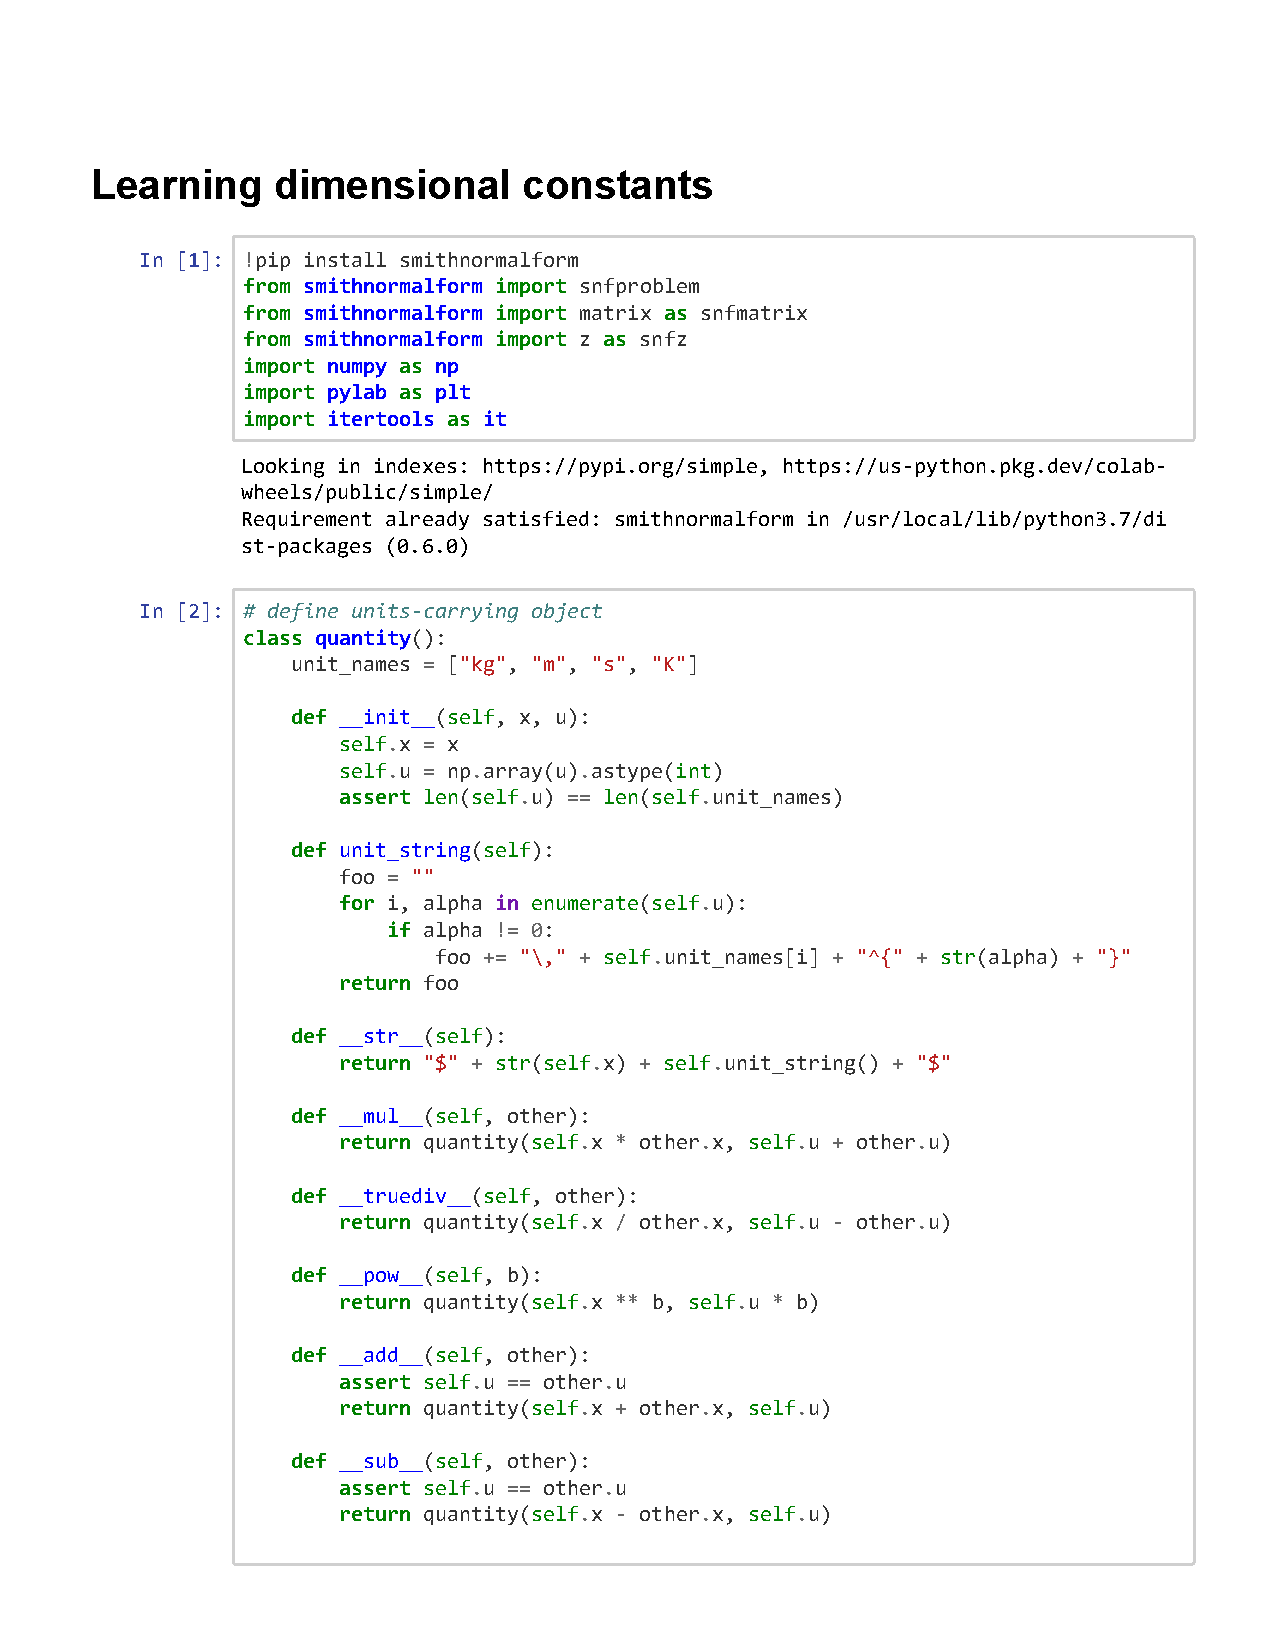
\includepdf[pages=1-12]{Learn dimensional constants.ipynb - Colaboratory.pdf}


\end{document}

% IT'S OVER
% ------------------------------------
% \section{DELETE THIS SECTION: Discussion and other random notes}

% Four special cases:
% \begin{enumerate}
%     \item the representation that retains dimensions but drops all numbers --- here the structure $\rho(g)$ is the graded algebra of dimensions...
%     \item the representation that discards all dimensions and just describes transformations of numerical quantities
%     \item a statistical representation --- here, $g$ could be 'prediction', and we may for instance want a $\Phi$ which makes prediction statistically or computationally easier
%     \item a causal representation --- here, $g$ could be a class of interventions, possibly described by a group (e.g., translations of objects)
% \end{enumerate}

% xxx could also talk about equivariance with respect to sample size. Statistical inference procedures should be expressed s.t.\ they work independent of sample size

% Approximate symmetries and representations that are approximate.

% Any connection between this stuff and causality?
% Example of cannon ball where influence of $m$ can be ruled out based on dimensional analysis --- write an SCM: (1) two variables are the initial values of $v$, $m$, chosen independently, and the final value of $l$ (2) $g$ is considered constant, (3) $\theta$ is the noise affecting $l$. From time constraints we know that the only possible causal arrows are from $v, m$ to $l$. From dimensional analysis, the arrow $m\to l$ is excluded, so we have identified the causal graph $v\to l$.


